% !TeX root = RJwrapper.tex
\title{A Hexagon Tile Map Algorithm for Displaying Spatial Data}
\author{by Stephanie Kobakian, Dianne Cook, and Earl Duncan}

\maketitle

\abstract{%
Spatial distributions have been presented on alternative representations
of geography for many years. In modern times, interactivity and
animation have allowed alternative displays to play a larger role.
Alternative representations have been popularised by online news sites,
and digital atlases with a focus on public consumption. Applications are
increasingly widespread, especially in the areas of disease mapping, and
election results. The algorithm presented creates a display that uses
tessellated hexagons to represent a set of spatial polygons. It
allocates these hexagon in a manner that preserves the spatial
relationship of the geographic units, in light of their positions to
points of interest. The display showcases spatial distributions, by
emphasising the small geographical regions that are often difficult to
locate on geographic maps.
}

\hypertarget{introduction}{%
\subsection{Introduction}\label{introduction}}

Many cancer atlases present geospatial cancer data on a choropleth map
display. The Australian Cancer Atlas \citep{TACA} is a recent addition
to the many cancer atlas maps worldwide. The ground-breaking atlas for
Australia presents a central map that shows the landmass overlaid with
administrative boundaries. This choropleth display can highlight the
geographic patterns in geospatially related cancer statistics
\citep{SAMGIS}.

Over time, the density of living in major cities has increased as
residents have gathered to live near urban areas \citep{ACTUC}. The
division of these residents into approximately equal population areas
results in dramatically different square meterage of administrative
geographic units, such as states or electorates. In a choropleth map
display, the geographic units are coloured to represent the value of the
statistic for each unit \citep{EI}. This can cause some values to be
emphasised over others, and allows choropleth map displays to
misrepresent the spatial distributions of human related statistics due
to area-size bias \citep{BCM}. Figure \ref{fig:choro} is a choropleth
map that uses colour to display the estimated standardised incidence
ratios (SIRs) of thyroid cancer for females, in each of the Statistical
Areas at Level 2 (SA2) used by the \citet{abs2011}. The Australian
choropleth map display draws attention to the expanse of dark and light
blue areas across the rural communities in all states. The SA2s on the
east coast around Brisbane and in northern New South Wales stand out as
more orange and red. However, this display neglects the vast amount of
Australia residents living in the densely populated capital cities.

\begin{Schunk}
\begin{figure}
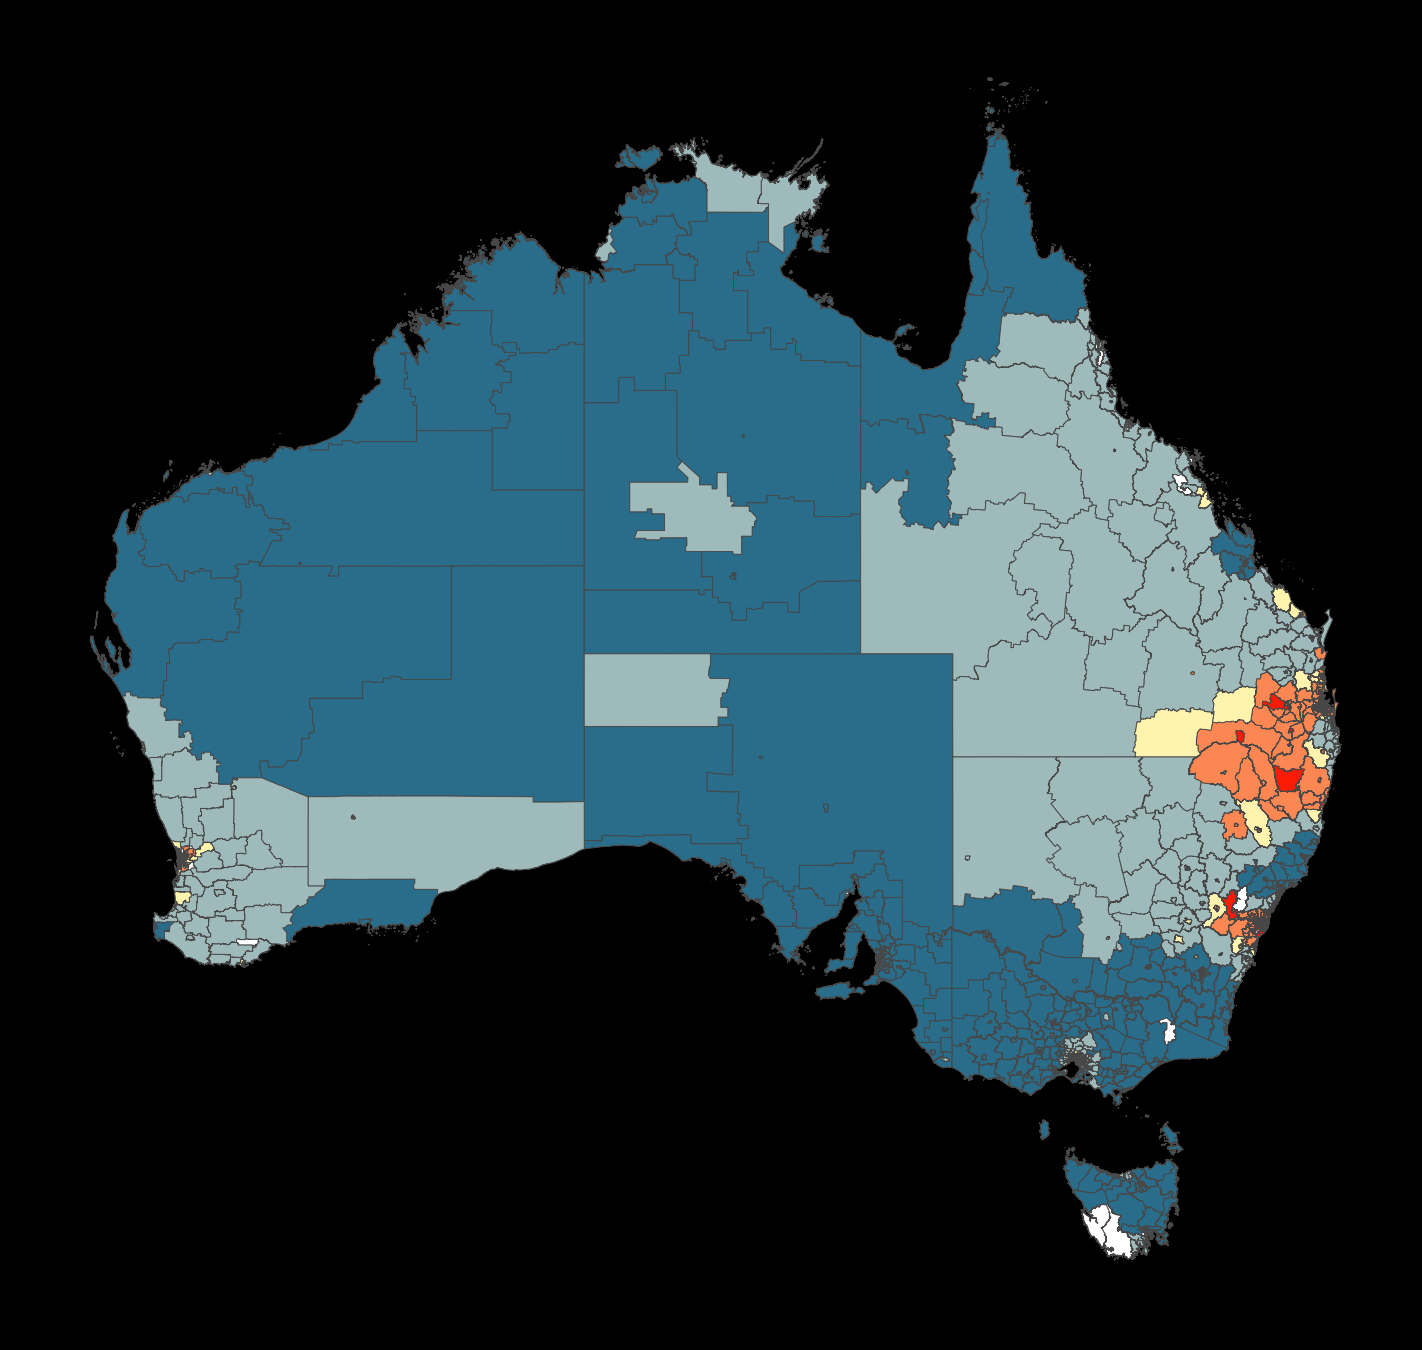
\includegraphics[width=0.95\linewidth]{kobakian-cook_files/figure-latex/choro-1} \caption[A choropleth map of thyroid incidence among females across the Statistical Areas of Australia at Level 2]{A choropleth map of thyroid incidence among females across the Statistical Areas of Australia at Level 2. Blue indicates lower than average and red indicates higher than average incidence. A cluster of high incidence is visible on the east coast.}\label{fig:choro}
\end{figure}
\end{Schunk}

The solutions to this visualisation problem begin with the geography.
Alternative maps can be created to shift the focus from land area and
shape to the value of the statistics \citep{ACCAC}. Each style of
cartogram applies a different transformation to the geographic areas, to
highlight the values of the statistic of interest. Alternative maps can
result in a distortion of the map space to represent features of the
distribution across the areas \citep{ACCAC} as the statistic of interest
is used to determine the cartogram layout.

Alternative mapping methods allow increased understanding of the spatial
distribution of a variable across the population, by fairly representing
the population in each administrative area \citep{TAAM}. This
acknowledges that the number of residents can be different and also
recognises that each area, or person within it is equally important.

This paper contains a discussion of Existing Mapping Practices. This is
followed by details of the Algorithm. The implementation section
discusses the algorithm in the \texttt{sugarbag} package. Finally, the
use and benefits of animation are presented.

\hypertarget{existing-mapping-practices}{%
\subsection{Existing Mapping
Practices}\label{existing-mapping-practices}}

The familiar choropleth map display is often used to allow the user to
orient themselves. However, the emphasis on the land mass diminishes the
features of the distribution in densely populated communities due to the
small size on the display \citep{ACTUC}. The unique shapes of boundaries
can be helpful for orienting users but may not contribute to their
understanding of the spatial disease distribution as many of the
communities are not visible in a choropleth display \citep{TVSSS}.

Administrative areas are often used to aggregate census data and used to
understand demographics within communities of the Australian population.
Each SA2 \citep{abs2011} was designed to represent a community. This
collection of communities presents an opportunity for explicit map
transformations to improve communication of spatial distributions
\citep{CBATCC}. In figure \ref{fig:tas_displays} the choropleth map can
be seen underneath each alternative map display to allow for comparisons
to be made.

There are several established alternative visualisation methods. Tile
maps, rectangular cartograms \citep{ORC} and Dorling cartograms
\citep{ACTUC} all use one simple shape to represent each geographic
unit. They all minimise the emphasis on the size or shape of the
geographic areas. These alternative map displays focus on the
relationship between neighbours, attempting to preserve connections, and
disregard the unique shapes of the administrative boundaries. Figure
\ref{fig:tas_displays} shows a collection of alternative map displays,
this includes a) a contiguous cartogram, b) a non-contiguous cartogram,
and c) a Dorling cartogram.

\begin{Schunk}
\begin{figure}
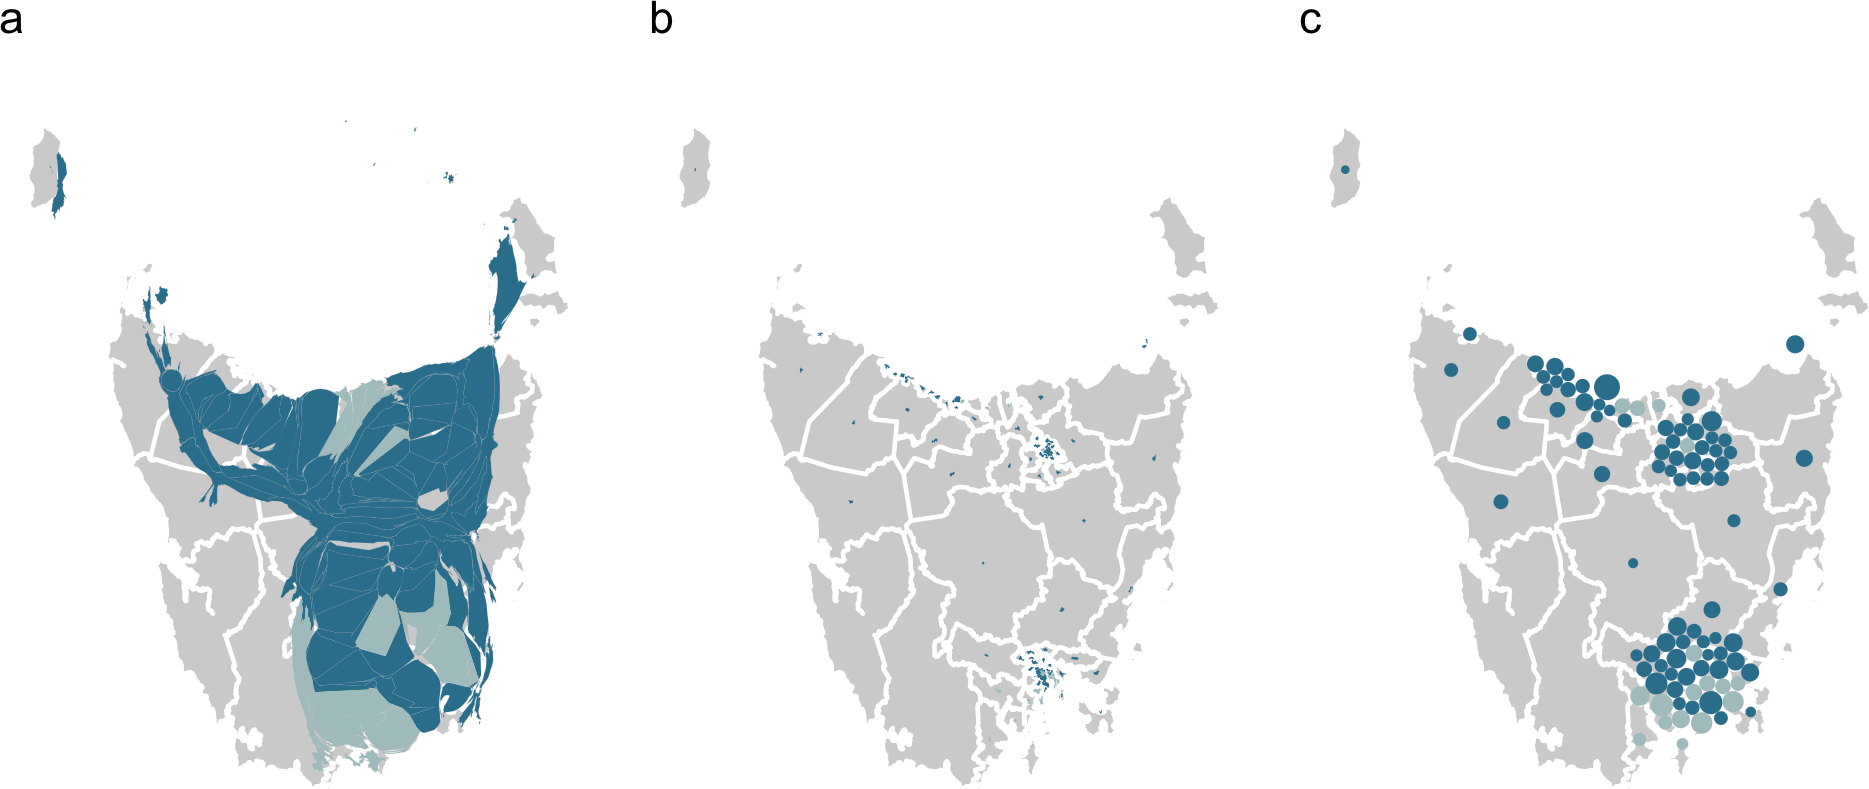
\includegraphics[width=0.95\linewidth]{kobakian-cook_files/figure-latex/tas_displays-1} \caption[The three displays show alternative maps of the Australian state of Tasmania at SA2 level]{The three displays show alternative maps of the Australian state of Tasmania at SA2 level: (a) contiguous cartogram, (b) non-contiguous cartogram and (c) Dorling cartogram of Tasmania. The contiguous cartogram looks like the state has an hourglass figure, while the non-contiguous cartogram shrinks areas into invisibility. The Dorling expands the metropolitan regions.}\label{fig:tas_displays}
\end{figure}
\end{Schunk}

When communicating information that is relevant to the population, each
member of the population can be given equal representation by
transforming the map \citep{TVSSS}. The connected communities can be
recognised by allowing the boundaries to maintain connection in the
transformed display. The contiguous cartogram displayed in figure
\ref{fig:tas_displays}a) draws attention to smaller geographic units
when they are rescaled according to the population \citep{DMAHP}. These
new shapes can now be coloured to represent a second variable. The
algorithm uses the geographic shape of the areas and iterates toward
sizing the areas to represent the population. This display can create
twisted and unfamiliar shapes from the geographic units as the
algorithms must satisfy the topology conditions, especially when there
are communities located geographically far from their neighbours
\citep{TVSSS}.

The non-contiguous cartogram in figure \ref{fig:tas_displays}b) also
uses the population to rescale the geographic units. Unlike the
contiguous cartogram, the SA2 areas maintain their geographic shape, but
they may not retain the connection with their neighbours. The population
of the SA2 areas is used to scale the geographic units in the
non-contiguous cartogram \citep{NAC}. The amount of background space can
be meaningful in non-contiguous cartograms \citep{ECGC}. The size
disparity between rural areas and urban areas result in reasonable
display within the south eastern city of Hobart, but these units are not
visible in the context of the Tasmania state map. Depending on the
difference between the population and geographic land size, the amount
of white space can also prevent meaningful understanding of the
distribution \citep{TVSSS}.

The Dorling cartogram presents each geographic unit as a circle, the
size of the circle is scaled according to the population value of each
area \citep{ACTUC}. Figure \ref{fig:tas_displays}c) shows the Tasmania
SA2 areas as an individual circle located as close as possible to the
geographic centroid location. This map draws attention to the collection
of coastal cities in Tasmania that were not apparent in Figure
\ref{fig:tas_displays} a), or b). This display also highlights that the
approximation of equal population is not easy to fulfil, as there is
some disparity in the sizes of the circles.

\hypertarget{algorithm}{%
\subsection{Algorithm}\label{algorithm}}

The purpose of this algorithm is to create an alternative map display
that highlights the spatial distributions for populations. There has
been an increasing need for displays that recognise the large number of
people that live in dense urban environments. The algorithm intends to
maintain the spatial relationships of a group of geographic units using
the relationship between each unit and the closest focal point. The
algorithm allocates geographic units to a representative hexagon, in
order of their proximity to the closest focal point.

The algorithm is implemented in the \texttt{sugarbag} package for
\texttt{R}, named after the common name for the \emph{Trigona
carbonaria} bee -- a species which builds flat layers of hexagonal brood
cells, spiralling out from a central point \citep{PH}. This unusual
pattern also provided the inspiration for the algorithm, where the maps
are constructed by building out from multiple focal points on the
geographic map base in a spiral fashion.

The result of the algorithm applied to the same data represented in
figure \ref{fig:choro} shows rates of thyroid cancer for females in each
of the SA2 areas of Australia as hexagons in figure \ref{fig:hexmap}.
The difference to the choropleth map in figure \ref{fig:choro} are
clear. Now the higher thyroid cancer incidence in the densely populated
areas in Sydney, Brisbane and Perth are visible. Interestingly, there is
no clear divide between rural and urban SA2 areas, as many rural areas
and the cities of Melbourne, Darwin, Adelaide and Hobart have low rates
of thyroid incidence for females. The hexagon tile map display provides
a more accurate representation of the spatial distribution of thyroid
cancer incidence across Australia.

Figure \ref{fig:hexmap} highlights the density of Australian capital
cities, as it draws attention to the many communities in Sydney,
Melbourne and Hobart. This display also highlights the disparity in the
burden of thyroid cancer for females in the communities of these cities.
There are several collections of red hexagons in Sydney that represent
the communities with much higher rates of diagnosis than the Australian
average. Brisbane also experiences higher than average rates of
diagnosis, but has more orange than red. The females in the cities of
Adelaide and Perth show much lower rates of diagnosis.

Compared to the choropleth map display in figure \ref{fig:choro}, the
low rates in the rural Australian communities are no longer dominating
the display. While the representative hexagons are still visible against
the black background, the much lower than average rates in rural
Australia are less noticeable.

\begin{Schunk}
\begin{figure}
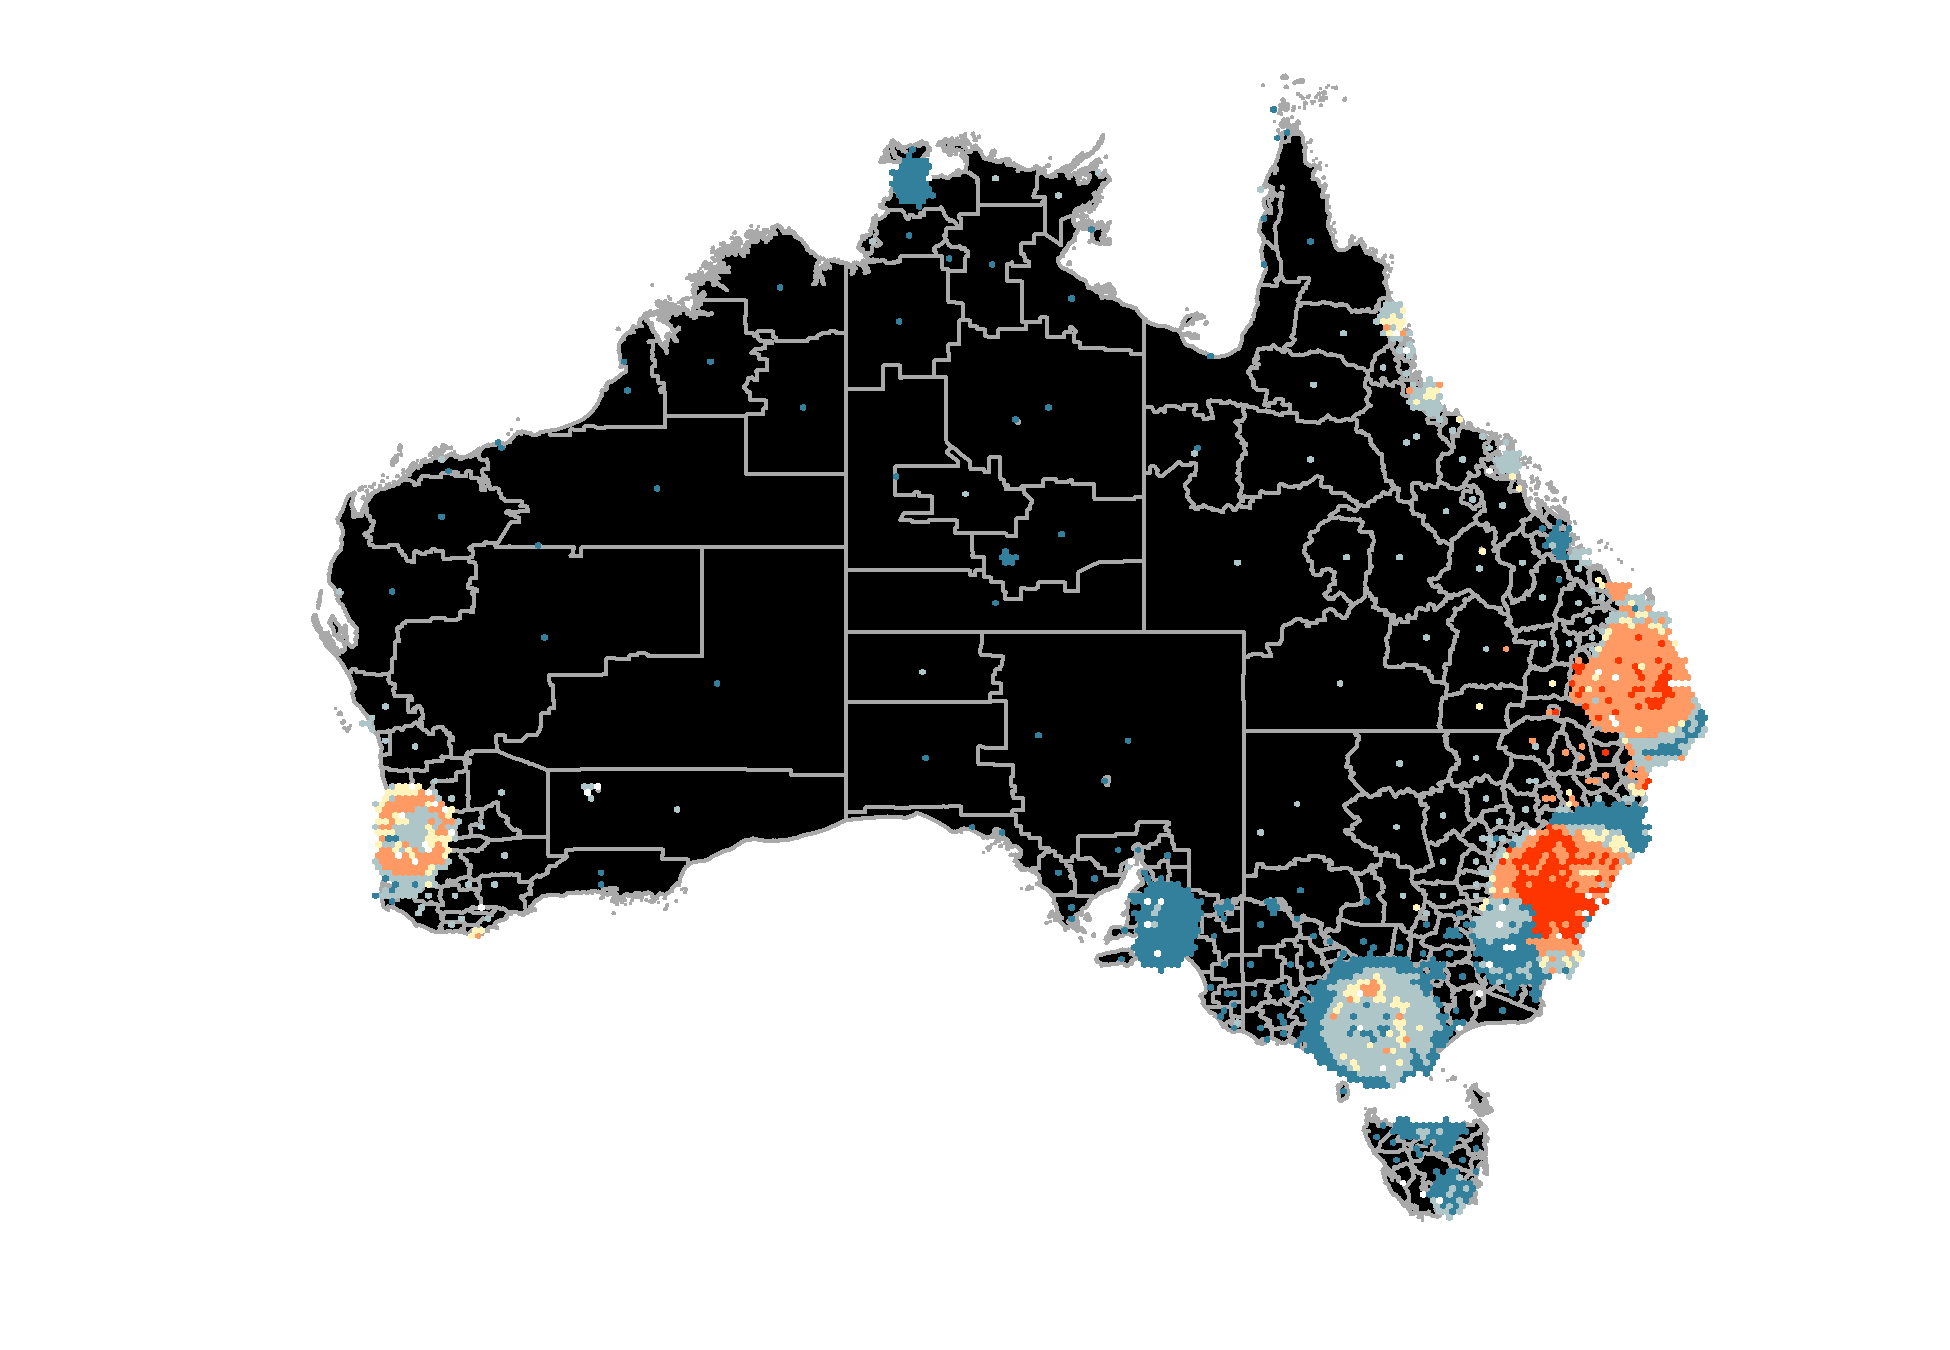
\includegraphics[width=0.95\linewidth]{kobakian-cook_files/figure-latex/hexmap-1} \caption[A hexagon tile map of female tyroid cancer incidence in Australia, the same data as shown in the choropleth map in Figure 1]{A hexagon tile map of female tyroid cancer incidence in Australia, the same data as shown in the choropleth map in Figure 1. The high incidence in several of the metropolitan regions (Brisbane, Sydney and Perth) can now be seen, along with numerous isolated spots.}\label{fig:hexmap}
\end{figure}
\end{Schunk}

There are several key steps in the creation of the hexagon tile map as
described in the flow chart in figure \ref{fig:sugarbag_flow}. First,
derive the set of centroids from the polygons provided, then create the
grid of hexagon locations. These two processes are defined in the blue
left column of the flow chart in figure \ref{fig:sugarbag_flow}. Each
centroid can then be allocated to an available hexagon location. The
steps for the allocation process are detailed in the right column of
figure \ref{fig:sugarbag_flow}. There are several filter steps to speed
the process of selecting an appropriate hexagon to represent each
geographic unit. To make tessellated plots with the hexagon allocations,
the point locations are converted into hexagon shapes.

\begin{figure}
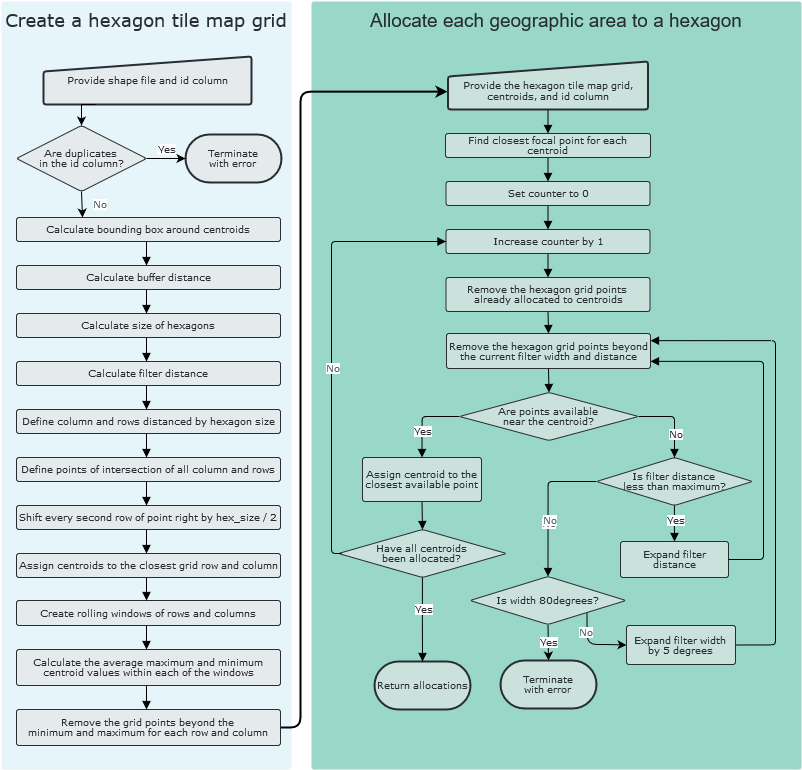
\includegraphics[width=14cm]{figs/sugarbag flow.png}
\caption{\label{fig:sugarbag_flow}A flow diagram detailing the steps taken to create a hexagon tile map. There are two basic processes, one to make the grid, and the other to allocate centroids to grid points.}
\end{figure}

\hypertarget{user-choices}{%
\subsubsection{User choices}\label{user-choices}}

Only two inputs are necessary to begin the algorithm; the shapefile, and
the ID variable. The ID variable should uniquely identify each
geographic unit in the shapefile.

The centroids are derived from the shapefile. The amount of centroids
within the geographic map is used to determine an appropriate hexagon
size if one is not provided. The derived centroids are a necessary input
for an appropriate grid to be constructed. Each grid point is located a
hexagon size distance from the next closest point in all six directions.
The grid will initially cover the entire map space, encompassing all the
centroid locations and will extend in all directions to the extent of
the buffer distance. This buffer distance can be helpful to account for
densely populated coastal areas, allowing the hexagon locations to
spread beyond the coastline, over the sea.

The centroid set and hexagon tile map grid are necessary for the
allocation process. Additionally, a set of reference locations can be
provided as focal points, typically compact and/or densely populated
areas such as major cities. The algorithm will use the focal points to
create the order of allocation, prioritising the closest centroid
locations to the focal points. The user can also specify the variable
that should be used to determine the order for the allocation.

When allocating representative hexagons, the width parameter can be used
to determine the flexibility of positioning. Using the relationship with
the nearest focal point, a larger width parameter will increase the
amount of available hexagons nearer to the original centroid of the
geographic unit. A smaller width will maintain the orientation from the
focal point to the centroid when selecting the hexagon location.
However, this could mean it is placed further away.

\hypertarget{implementation}{%
\subsection{Implementation}\label{implementation}}

Hexagon tile maps can be useful to understand a distribution across a
collection of geographic areas. However, these maps are not easy to
create manually, especially as the number of areas increases. This
algorithm was created to automate this process, and reduce the manual
load involved in creating and implementing alternative displays. This
allows map makers and data communicators to spend their time choosing
the most effective display.

The \texttt{sugarbag} package contains a set of functions that help R
users to create a hexagon tile map. The algorithm presented in the
\texttt{sugarbag} package operates on a set of simple feature geometry
objects , known as \texttt{sf} objects\citep{sf}. This package allows R
users to create \texttt{sf} objects by importing polygons stored in
various formats. Users should provide a set of polygons that define
geographic units by their administrative boundaries. The functions
arrange the geographic units in order of proximity to a set of locations
provided, such as the centre of major cities. The centroid location of
each geographic unit is used to measure the proximity. It emphasises the
major cities as population hubs, rather than emphasizing the size of
large, rural geographic units.

A user can tweak the parameters of the hexagon map using the additional
arguments to the \texttt{create\_hexmap} function, but these options may
affect the speed of the algorithm. The hexagon size may need adjustments
depending on the density of the population; users can provide an
appropriate hexagon size and re-run the algorithm. The buffer distance
may need to be increased if the coastal cities need to extend beyond the
geographic land mass.

\hypertarget{algorithm-steps}{%
\subsection{Algorithm steps}\label{algorithm-steps}}

The package can be installed from CRAN:

\begin{Schunk}
\begin{Sinput}
install.packages("sugarbag")
\end{Sinput}
\end{Schunk}

and the development version can be installed from the GitHub repository:

\begin{Schunk}
\begin{Sinput}
devtools::install_github("srkobakian","sugarbag")
\end{Sinput}
\end{Schunk}

The following steps create the hexagon tile map for all the Statistical
Areas at Level 2 in Tasmania. These steps can be executed by the main
function, \texttt{create\_hexmap}, or can be run separately for more
flexibility.

If a user would like to perform each of the steps of the algorithm
themselves, the necessary inputs will change for each function. For
example, the \texttt{allocate} function can be used directly when a user
wishes to use a set of centroids, rather than polygons.

The set of SA2 polygons for Tasmania, using the 2011 definition of SA2s,
is accessed from the \texttt{absmapsdata} package. A single column of
the data set is used to identify the unique areas. In this case, the
unique SA2 names for each SA2 have been used.

The Australian capital cities are used as focal points to allocate each
geographic area around the closest capital city. Hobart will be the
focal point for this example because only the state of Tasmania is being
processed.

The buffer distance, hexagon size, hexagon amount to filter and width of
angle are parameters that will be determined within
\texttt{create\_hexmap()}, if they are not provided. They are created as
they are needed throughout the following example.

The results from various steps in the process are illustrated in Figure
5.

\hypertarget{step-1-derive-the-set-of-centroid-points}{%
\subsubsection{Step 1: Derive the set of centroid
points}\label{step-1-derive-the-set-of-centroid-points}}

The set of polygons should be provided as an \texttt{sf} object, this is
a data frame containing a \texttt{geometry} column. The
\texttt{read\_shape()} function can assist in creating this object for
use in \texttt{R}.

The centroids can be derived from an \texttt{sf} object using the
\texttt{create\_centroids()} function:

\hypertarget{step-2-create-the-hexagon-grid-points}{%
\subsubsection{Step 2: Create the hexagon grid
points}\label{step-2-create-the-hexagon-grid-points}}

A grid is created to allow tessellation of the hexagons that represent
the geographic units. For a hexagon tile map, the grid of possible
hexagon locations is made using the \texttt{create\_grid()} function. It
uses the centroids, the hexagon size and the buffer distance. Figure
\ref{fig:filterprocess}a) shows the initial locations of grid points
created for Tasmania.

\hypertarget{creating-a-tessellated-grid}{%
\paragraph{Creating a tessellated
grid}\label{creating-a-tessellated-grid}}

A set of longitude columns, and latitude rows are created to define the
locations of the hexagons. The distance between each row and column is
the size specified by \texttt{hex\_size}. Equally spaced columns are
created from the minimum longitude minus the buffer distance, up to the
maximum longitude plus the buffer distance. Similarly, the rows are
created from the latitude values and the buffer distance. A unique
hexagon location is created from all intersections of the longitude
columns and latitude rows. Figure \ref{fig:filterprocess}a shows the
hexagon grid after every second latitude row on the grid is shifted
right, by half of the hexagon size.

\hypertarget{filtering-the-grid}{%
\paragraph{Filtering the grid}\label{filtering-the-grid}}

Not all of the grid points will be used, especially if islands result in
a large grid space. To filter the grid for appropriate hexagon locations
for allocation, the \texttt{create\_grid} function will call the
\texttt{create\_buffer} function. It finds the grid points needed to
best capture the set of centroids on a hexagon tile map. Reducing the
buffer can help to decrease the amount of time taken, as there will be
less points over the water to consider for each centroid allocation.

The closest latitude row and longitude column are found for each
centroid location. Then rows and columns of centroids are divided into
20 groups. The amount of rows in each latitude group and the amount of
columns in each longitude group are used as the width of rolling
windows. The first rolling window step finds the minimum and maximum
centroid values within each of the sliding window groups of longitude
columns, and the groups of latitude rows. The second rolling window step
finds the average of the rolling minimum and maximum centroid values,
for the longitude columns and latitude rows.

The hexagon grid points are kept only if they fall within the rolling
average of the minimum and maximum centroid values after accounting for
the buffer distance, for each row and column of the grid. Figure
\ref{fig:filterprocess}b displays remaining hexagon grid points after
applying the buffer filter. The sparsely populated South-West region of
National Park has fewer points available in the water compared to the
South-East region near the city of Hobart.

\hypertarget{centroid-to-focal-point-distance}{%
\paragraph{Centroid to focal point
distance}\label{centroid-to-focal-point-distance}}

The distance is calculated between each centroid in the set, and each of
the focal points provided. The order for allocation is determined by the
distance between the polygon centroid and it's closest focal point. For
this example, this distance is only calculated for the capital city of
Hobart, represented in figure \ref{fig:filterprocess}c and d as a white
cross.

\hypertarget{step-3-allocate-each-centroid-to-a-hexagon-grid-point}{%
\subsubsection{Step 3: Allocate each centroid to a hexagon grid
point}\label{step-3-allocate-each-centroid-to-a-hexagon-grid-point}}

Allocation of all centroids requires the set of polygon centroids and
the hexagon map grid. The polygon centroids are ordered from the
centroid closest to the focal point(s), to the furthest. This will
preserve spatial relationships with the focal point, as the inner city
areas are allocated first and placed closest to the capital, the areas
that are further will then be accommodated. The following example
considers the first of the Statistical Areas at Level 2. Within the
algorithm, these steps are repeated for each polygon.

\hypertarget{filter-the-grid-for-unassigned-hexagon-points}{%
\paragraph{Filter the grid for unassigned hexagon
points}\label{filter-the-grid-for-unassigned-hexagon-points}}

The set of possible hexagon grid points reduces by one after each
centroid is allocated, then only the grid points that have not yet been
selected are considered. Keeping only the available hexagon points
prevents multiple geographic units from being allocated to the same
hexagon. This is demonstrated in figure \ref{fig:filterprocess}c and d
by the black hexagons that represent the seven closest polygons to the
capital city of Hobart. As the allocation process begins for the eighth
closest centroid there are seven unavailable hexagon locations.

\hypertarget{filter-the-grid-points-for-those-closest-to-the-centroid}{%
\paragraph{Filter the grid points for those closest to the
centroid}\label{filter-the-grid-points-for-those-closest-to-the-centroid}}

A selection of possible hexagon locations around the centroid allows
only the closest points that are not yet assigned to be considered. The
number of possible hexagon locations to consider for a centroid is
determined by the \texttt{hex\_filter}. This is the maximum amount of
hexagons between the centroid and the furthest considered hexagon. It is
used to subset possible grid points to only those surrounding the
polygon centroid within an appropriate range. A smaller distance will
increase speed, but can decrease accuracy when width of the angle
increases.

The algorithm creates a circle of points, by only keeping points within
a certain radial distance around the original centroid location.

The \texttt{width} parameter is used to take a slice of the remaining
points. The width is the amount of degrees used on either side of the
angle from the focal point to centroid location. This uses the angle
from the closest capital city, to the current centroid as seen in figure
\ref{fig:filterprocess}c.~This allows the spatial relationship to be
preserved, even when it is allocated to a hexagon that is further from
the focal point then the original centroid location.

\begin{Schunk}
\begin{figure}
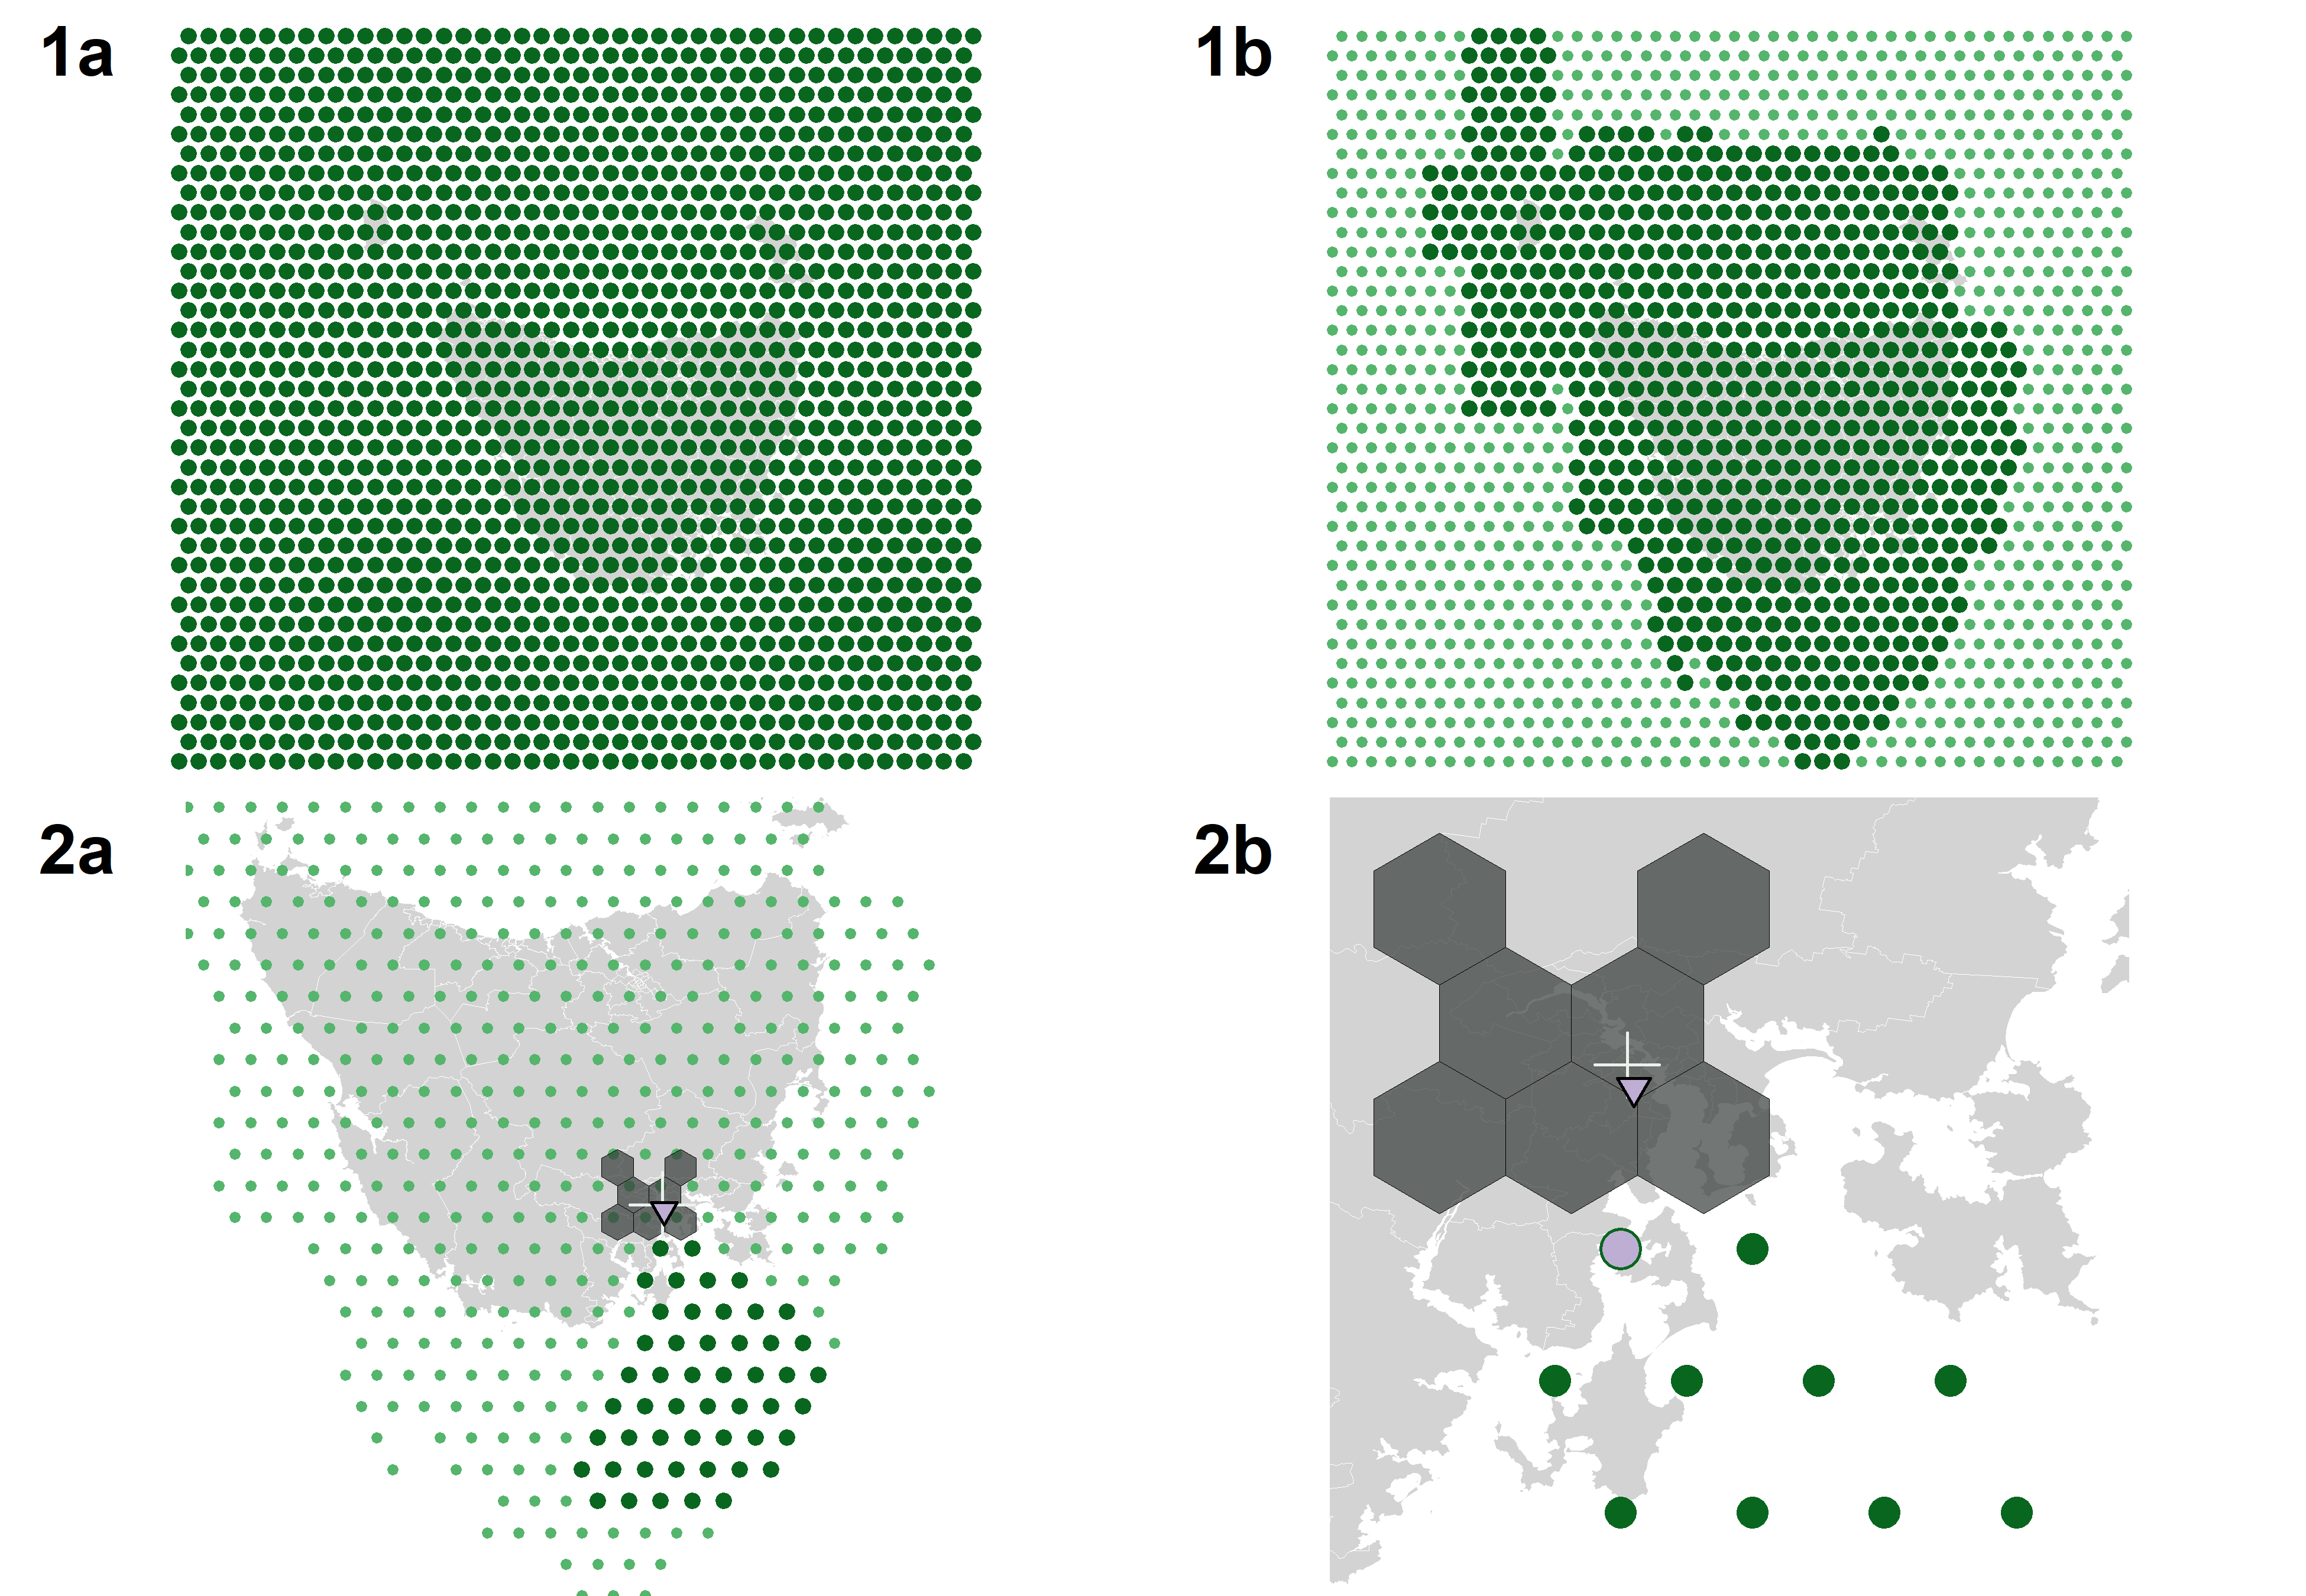
\includegraphics[width=0.95\linewidth]{kobakian-cook_files/figure-latex/filterprocess-1} \caption[Illustration of several steps of the algorithm]{Illustration of several steps of the algorithm: (a) ... (b) ... (c) ... (d). }\label{fig:filterprocess}
\end{figure}
\end{Schunk}

If no available hexagon grid point is found within the original filter
distance and angle, the distance is expanded and only when a maximum
distance is reached will the angle expand to accommodate more possible
grid points. By default the angle filter for the hexagon grid points
create plus and minus 30 degree bounds of the angle from the focal point
to the geographic centroid. This will increase if no points can be found
within the \texttt{hex\_filter} distance. The default angle of 30 was
chosen to allow the algorithm to find hexagons that best maintained the
spatial relationship between the focal point and geographic centroid.

\hypertarget{animation}{%
\subsection{Animation}\label{animation}}

Creating an animation connecting these two displays can allow users to
grasp the meaning of the connected hexagons. It will also highlight the
density of the communities using the rapid expansion of the inner-city
areas, these hexagons will move the furthest and will move rapidly in
the animation from their geographic locations. The rapid decrease in
size of the large rural areas can show the large size of their
collective landmass. The \texttt{gganimate} \citep{gganimate} package
can be used to make an animation. It connects the polygons for each area
in the two displays using the \texttt{sf\_id} variable, the names of the
statistical areas, and creates intermediate displays as they geographic
areas shrink or expand to the chosen hexagon size.

\hypertarget{conclusion-03}{%
\subsection{Discussion and Conclusion}\label{conclusion-03}}

This paper provides an algorithm for Australia called the hexagon tile
map. It also describes how this algorithm addresses the potential issues
found with contiguous, non-contiguous and Dorling cartograms when
applied to Australia. It achieves a display that effectively presents
the density of the population in small geographic areas and de
emphasises the large rural geographic space between the densely
populated capital cities.

The hexagon tile map display acknowledges that the amount of residents
can differ but each administrative area is equally important. This
solution uses equally sized areas, and maintain neighbourhood boundary
connections. The \texttt{sugarbag} package for \texttt{R} automates the
creation of tessellated hexagon tile maps by providing an algorithm to
design these displays. The Australian application preserves spatial
relationships, and emphasises capital cities. However, similar to the
choropleth map display the tessellation does not allow the size of the
hexagons to represent another variable. The algorithm is heavily
dependent on the focal points used, as this determines the order of
allocation. With careful consideration of the choropleth map, the small
geographic inner city areas may not have been noticed by viewers, but
the hexagon tile map display emphasises them. The communities in
northern Tasmania and the Northern territory do not draw attention
because of their size as in the choropleth, but their colour is still
noticeably below average when contrasted with the hexagons in New South
Wales.

This algorithm should be general enough to apply to other study regions
and contexts. The algorithm has only been tested using single countries.
While the buffer allows extension beyond the furthest centroids, there
is no mechanism implemented to protect the borders and ensure centroids
are placed within the geographic borders of a country. The algorithm is
also currently limited to representing each geographic area with only
one hexagon. Future developments may address these limitations, and
refine the filter steps for final selection of a hexagon grid point for
each centroid. A direct angle is currently implemented, but may narrowly
miss appropriate hexagons, a logarithmic function may help to choose a
closer hexagon to the original centroid location. This algorithm is an
effective start to creating hexagon tile maps for many geographic units.
This contributes to an extensive body of work that encourages the use of
alternative map displays for statistical displays of spatial data.

\bibliography{kobakian-cook.bib}

\address{%
Stephanie Kobakian\\
Monash University\\%
Department of Econometrics and Business Statistics\\
%
%
%
\\\href{mailto:stephanie.kobakian@monash.edu}{\nolinkurl{stephanie.kobakian@monash.edu}}
}

\address{%
Dianne Cook\\
Monash University\\%
Department of Econometrics and Business Statistics\\
%
%
%
\\\href{mailto:dicook@monash.edu}{\nolinkurl{dicook@monash.edu}}
}

\address{%
Earl Duncan\\
Queensland University of Technology\\%
School of Mathematical Sciences\\
%
%
%
\\\href{mailto:earl.duncan@qut.edu.au}{\nolinkurl{earl.duncan@qut.edu.au}}
}

